\section{App implementation}\label{ch:app_implementation}

The prototype suffices as proof of concept.
However, the model lacks a suitable environment to be used.
The prototype applies the model and its implementation into each instance of \name{mec-2} and patches a canvas on top of the element to be able to draw.
This is not optimal, because this approach is neither flexible nor extensible.
So instead of using just the \name{mec2} HTML-element, a web application is built around it.
This web application may be used as a progressive web app to be accessed via a browser or even embedded into other third-party frameworks.

\subsection{Creation of a Progressive Web App}

The goal of the application is to provide a user interface for the user to work with \name{mec2} interactively.
The application should be designed to be extensible to allow other means of interacting with \name{mec2}; for example using hand-drawings.
This is achieved by using \name{mec2} as the base and creating an environment around this HTML-element.

Components used to create the user interface are mostly written using \name{React}. % TODO citation needed.
React is a JavaScript framework, which allows for the usage of single components, allowing standard HTML and JavaScript besides it.
This is a requirement the original \name{mec2} HTML-Component should be used without any modifications.
By using the \name{materialUI}\cite{MaterialUI2020} a consistent and modern layout is created.

\subsection{Structure of the application}

\begin{figure}
    \centering
    \fbox{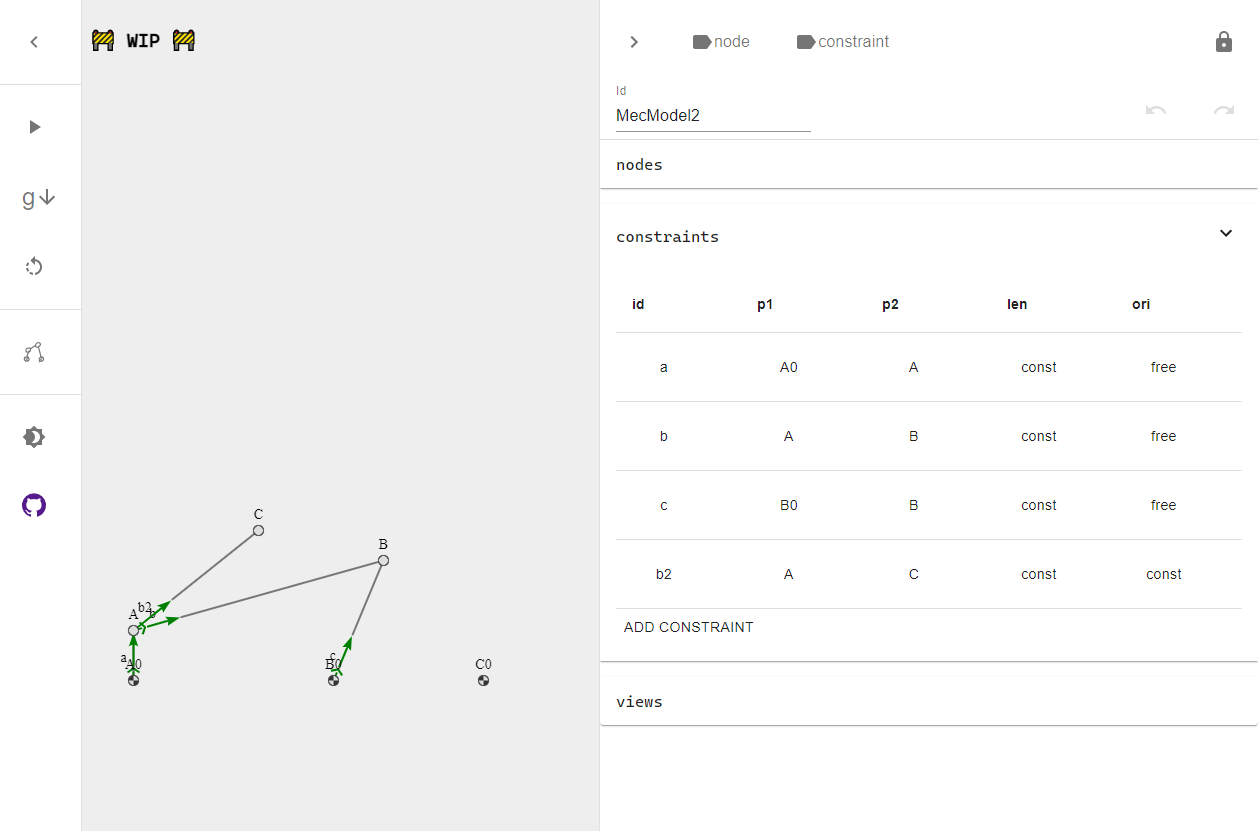
\includegraphics[width=0.8\textwidth]{images/deepmech_klawr_de.png}}
    \caption[Screenshot of the web application]{ Both drawers are expanded. On the left the \name{mec2} controls can be seen, on the right a summary of elements of the model are listed. The tab for \name{constraints} is expanded where some properties are shown }\label{fig:deepmech_klawr_de}
\end{figure}

The main part of the application is occupied by the \name{mec2} Custom HTML element.
It is stretched across the whole viewport.
On both sides are \name{Material-UI} \code{Drawer} elements, enabling the user to interact with different parts of the application.

The structure of the user interface aims to be simple and straight forward.
To define individual components \name{Reacts} \name{jsx} syntax is used.
\name{jsx} is a syntax very similar to \name{HTML} but with the ability to implement JavaScript into the elements\footnote{By using \name{jsx} it is now necessary to compile the project using \name{Babel.js}.}. % TODO citation neede

\subsubsection{Left drawer}

The left drawer contains \code{MecControl}, \code{DeepmechControl} and two other Buttons.
\code{MecControl} is a custom \name{React} component to replace the default \name{mec2} controls by using the designated API.\@

\begin{lstlisting}[label={lst:mec_control}, caption={Definition of the \name{MecControl} component.}]
export default function MecControl({ mecReset, className }) {
    const dispatch = useDispatch();
    const mec = useSelector(mecSelect);

    return <List className={className}>
        <ListButton onClick={() =>
            dispatch(mecAction.toggleRun())} tooltip="Run/Pause mechanism">
            {mec.pausing ? <PlayArrow /> : <Pause />}
        </ListButton>
        <ListButton onClick={() =>
            dispatch(mecAction.toggleGravity())} tooltip="Toggle gravity">
            g {mec.gravity ? <Clear /> : <ArrowDownward />}
        </ListButton>
        <ListButton onClick={mecReset} tooltip="Reset">
            <RotateLeft />
        </ListButton>
    </List>
}
\end{lstlisting}

Listing~\ref{lst:mec_control} shows the function which returns the component replacing the default \name{mec2} controls.
It contains the definition of the variables \code{dispatch} and \code{mec}.
\code{Selector} and \code{useDispatch} are used for state management of the user interface and are examined in Chapter~\ref{ch:state_manipulation}.
The return value of a component is the contonent defined in \name{jsx} syntax.
\code{List} is a \name{Material-UI} component.
The list items inside the list are are implemented using \code{ListItems} containing a \code{Tooltip} and an \code{IconButton}.
To reuse \name{Material-UI} components multiple times without calling them every time a custom \code{ListButton} component is created.
The \code{ListButton} is a combination of the \code{ListItem}, \code{Tooltip} and \code{IconButton} components and can be reviewed at \aka{https://github.com/klawr/deepmech/blob/gh-pages/src/Components/Utils/ListButton.js}.

The left drawer also contains the \code{DeepmechControl}\footnote{\name{deepmech} is the current project name.}.
It is responsible for handling the draw mode.
It only shows the activation button if the draw mode is disabled.
If the drawing mode is enabled the left drawer does not show the \code{MecControl} anymore.
Furthermore, the \code{DeepmechControl} shows four different modes interacting with the drawing canvas: drawing, panning and deletion of line strokes and a camera mode, which is not implemented yet.
Details of the different modes and how they are implemented are explained in Chapter~\ref{ch:state_manipulation}.

The two bottom-most buttons are responsible for toggling the dark-mode\footnote{The app starts in dark mode if the executing browser is in dark-mode, and vice versa.} and to navigate to the project page: \url{https://github.com/klawr/deepmech}.

\subsubsection{Right drawer}

The drawer on the right side intends to show all relevant information of the \name{mec2} model.
On the top, there are two buttons labeled \code{nodes} and \code{constraints} each with a \code{Label} icon.
Those are used to toggle the labels of \code{nodes} and \code{constraints} respectively.
The \code{Lock}-button is used to keep the drawer open when interacting with the model.
The right drawer is locked by default if the side is wide enough; i.e.\ wider than 1200 pixels.

The last component in the \code{RightDrawer} is the \code{MecProperties} component.
The \code{MecProperties} component contains a collection of other custom components.
Four properties of a \name{mec2} model have designated components.
The first component is the \code{Id} component.
It is showing the \code{id} property of the \name{mec2} model and updates it respectively on changes.

Currently, three of the modules provided by \name{mec2} are implemented into the app:
\code{Nodes}, \code{Constraints} and \code{Views}.
They are all structured in a very similar way to have a somewhat unified interface for the user.
To achieve this the return value of these components is very similar and can be seen in Listing~\ref{lst:mec_component_return}.

\begin{lstlisting}[label={lst:mec_component_return}, caption={Return value of a custom \name{mec2} component.}]
return <Accordion>
    <AccordionSummary> {name} </AccordionSummary>
    <AccordionDetails>
        <Grid container direction="row">
            <MultiSelect options={head} updateOptions={updateHead} />
            <MecTable
                SanitizedCell={SanitizedCell}
                head={Object.entries(head).filter(h => h[1]).map(h => h[0])}
                list={mecElement._model[name]} />
        </Grid>
    </AccordionDetails>
</Accordion>
\end{lstlisting}

The \code{Accordion} in this listing is a \name{Material-UI} component\footnote{\aka{https://material-ui.com/components/accordion/}}.
This component accepts the \code{AccordionSummary} and \code{AccordionDetails}, which are defined inside the \code{Accordion}.
In Listing~\ref{lst:mec_component_return} the \code{AccordionSummary} encapsulates the \code{name} property of the respective component, which is the name of the component in lower case; e.g. \code{const name = 'nodes'} for the \code{Nodes} component.
\code{AccordionDetails} contains elements that are shown when the \code{Accordion} is expanded.

The \code{AccordionDetails} component shows details of the respective property of the \name{mec2} model.
The \code{Grid} in the \code{AccordionDetails} in~\ref{lst:mec_component_return} contains two custom components.
\code{MultiSelect} is a dropdown menu which shows a list of the available properties of the module; e.g.\ for nodes these properties are \code{id}, \code{x}, \code{y}, \code{base}.
These properties are provided by the variable \code{head}, which is given inside the definition of the component.
This enables the possibility to show and modify other properties later on, without the necessity to show them from the start\footnote{To show all possible properties directly would also result in a very unclear user interface.}.
The \code{head} variable is a list of properties which is further discussed in Chapter~\ref{ch:state_mec2_model}.

The \code{MecTable} component is responsible for rendering the table where the properties are shown.
\code{MecTable} returns a predefined layout of a regular \code{Table} element of \name{Material-UI}, which can be reviewed at \aka{https://material-ui.com/components/tables/}.
The \code{TableHead} in \code{MecTable} contains a mapping of the different properties which are provided by \code{head} to show the properties which are shown by each column.
The rows of the table are filled using yet another custom component: \code{SanitizedCell}.
The \code{SanitizedCell} component is injected into the \code{MecTable}, wheras the definition of the component itself is provided by the encompassing component.
It provides information on how the individual properties are to be rendered.
The respective return value of the \code{SanitizedCell} function can be seen in Listing~\ref{lst:sanitized_cell}.

\begin{lstlisting}[label={lst:sanitized_cell}, caption={Return value of the \code{Node} components \code{SanitizedCell} function.}]
return <ContextMenu key={idx}>
    {select()}
    <MenuItem onClick={removeNode}>
        {`Remove node ${elm['id']}`}
    </MenuItem>
\end{lstlisting}

\code{select} returns the respective function based on a switch statement, which can be seen in~\ref{lst:sanitized_cell_select}.

\begin{lstlisting}[label={lst:sanitized_cell_select}, caption={\code{select} function in \code{SanitizedCell} of the \code{Node} component.}]
function select() {
    switch (property) {
        case 'base':
            const [checked, changeChecked] = React.useState(!!elm[property]);
            return <Checkbox checked={checked} onChange={(e) => {
                    changeChecked(e.target.checked);
                    update(e.target.checked);}} />
        case 'x':
        case 'y':
            return <UpdateText
                title={property}
                value={Math.round(elm[property])}
                onSubmit={v => update(+v)} />
        case 'id': /*...*/
        default: return <div>{elm[property]}</div>
}
\end{lstlisting}

\code{SanitizedCell} is called with an argument object containing \code{property}, \code{idx} and \code{elm}.
The \code{property} corresponds to the current value of \code{head}, which is mapped in the \code{MecTable} to fill the \code{TableRow}\footnote{Yet another property of \code{Table} which is responsible for the design of the table-rows.}.
Based on the \code{property} value the \code{select} function returns the component designed for the specific property.
If the property is equal to \code{'base'} the return value is \name{Material-UI}s \code{Checkbox}.
For textual inputs the custom component \code{UpdateText} is created, which handles updates reliably to be translated to the \name{mec2} model and back.
It is therefore used by number value like \code{'x'} and \code{'y'} or textual value like \code{'id'}.

Another custom component, which is used inside a \code{SanitizedCell} component is \code{RadioSelect}.
This custom component contains a selection of items and hold one as the selected item; e.g.\ constraints inside a \name{mec2} model reference two nodes, which are selected via their respective \code{id} property.
This component can list all nodes by their \code{id} property and select one respectively.

\subsubsection{The canvas}

As mentioned above, the viewport is occupied by the \name{mec2} Custom HTML element.
The prototype used the canvas of this HTML element to be able to draw.
This approach is cumbersome because the corresponding event handlers had to be activated and deactivated manually, which gives a lot of room for error and is not a very flexible approach.

In unison with the rest of the application, this canvas element modeled into a custom component.
The \code{DeepmechCanvas} component does not return a \name{React} component, but a HTML canvas, as demonstrated in Listing~\ref{lst:deepmech_canvas}.

\begin{lstlisting}[label={lst:deepmech_canvas}, caption={Return of the \code{DeepmechCanvas} component.}]
return <canvas
    id="{id}" className={classes.drawCanvas}
    width={globalThis.innerWidth} height={globalThis.innerHeight}
    ref={canvasRef} />
\end{lstlisting}

The \code{id} property is used to refer to this canvas from other components.
The \code{DeepmechControl} component uses this \code{id} to be able to get access to the canvas-HTML element and forwards it to the \code{predict} function.

\code{width} and \code{height} are taken from the \code{globalThis}\footnote{\aka{https://developer.mozilla.org/en-US/docs/Web/JavaScript/Reference/Global_Objects/globalThis}} property.

The \code{DeepmechCanvas} component has a \code{canvasRef} variable which is initially set to \code{const canvasRef = React.useRef(null)}.
Every time the \code{DeepmechCanvas} component is rendered the \code{canvasRef} is updated by the \code{ref} property of the returned HTML element.
See \aka{https://reactjs.org/docs/hooks-reference.html\#useref} for more information about \code{React.useRef}.

Because the reference is created after initialization, \name{Reacts} \code{useEffect}\footnote{\aka{https://reactjs.org/docs/hooks-reference.html\#useeffect}} has to be used.
\code{DeepmechCanvas}' \code{useEffect} is shown in Listing~\ref{lst:deepmech_canvas_use_effect}.

\begin{lstlisting}[label={lst:deepmech_canvas_use_effect}, caption={The \code{useEffect} function in the \code{DeepmechCanvas} component.}]
React.useEffect(() => {
    const [nl, cl] = [mec.nodeLabels, mec.constraintLabels];
    dispatch(mecAction.toggleNodelabels(false));
    dispatch(mecAction.toggleConstraintlabels(false));
    dispatch(UiAction.right(false));
    const ctx = canvasRef.current.getContext('2d');
    return handleInteractor(ctx, deepmech.mode, placeholder, () => {
        dispatch(mecAction.toggleNodelabels(nl));
        dispatch(mecAction.toggleConstraintlabels(cl));
    });
}, [deepmech.mode]);
\end{lstlisting}

The second argument (\code{[deepmech.model]}) is an array that defines properties on which changes are monitored.
Every time a change is registered, the function given as the first argument is issued.

The first argument given to this function is also called after the component is rendered the first time.
This behavior is necessary because the canvas has to be initialized for the context of the canvas element to be set via \code{canvasRef.current.getContext('2d')}.
The \code{dispatch} calls set certain values which will be further examined in Chapter~\ref{ch:state_manipulation}.
Returned is a \code{handleInteractor} function.

The \code{handleInteractor} function handles the interaction of the user with the canvas.
It creates a new instance on the \code{canvasInteractor}\footnote{The \code{canvasInteractor} is discussed in Chapter~\ref{ch:canvas_interactor}} for the given \code{ctx}.
As with \code{mec2}, the global \code{canvasInteractor} is used here.

For the selection of individual \name{g2}-elements a \code{selector} variable is set to \code{g2.selector(interactor.evt)}.
The respective event listeners are defined for five different events as described in Listing~\ref{lst:handle_interactor_event_listeners}.

\begin{lstlisting}[label={lst:handle_interactor_event_listeners}, caption={Definition of event listeners on the \code{canvasInteractor}.}]
const o = { tick, pointerdown, pointerup, drag, click: pointerup }
Object.entries(o).forEach(e => interactor.on(...e));
\end{lstlisting}

The event listeners have functions to handle events based on the current \code{mode} which is inserted by the function call\footnote{Every time the mode changes the function is called again, as described in the array which is given as the second argument to the \code{React.useEffect} function.}.

For example the \code{pointerdown} function, as described in Listing~\ref{lst:handle_interactor_pointerdown} contains a switch-statement handling events when the \code{mode} is set to \code{'draw'} or \code{'delete'}.

\begin{lstlisting}[label={lst:handle_interactor_pointerdown}, caption={\code{pointerdown} function in \code{handleInteractor}.}]
function pointerdown(e) {
    switch (mode) {
        case 'draw':
            // Set ply and add to command queue
            ply = {
                pts: [{ x: e.x, y: e.y }],
                lw: '2', ls: '#fff', lc: 'round', lj: 'round',
                get sh() { return this.state & g2.OVER ? plyShadow : false; }
            };
            placeholder.ply.ply(ply);
            break;
        case 'delete':
            // Filter selected node from commands array
            placeholder.ply.commands = placeholder.ply.commands.filter(
                cmd => cmd.a !== selector.selection);
            selector.evt.hit = false; // selector gets confused
            selector.selection = false; // overwrite selection
            break;
    }
}
\end{lstlisting}

% TODO have I talked about the placeholder to fill the mec element? 

The \code{ply} variable is a placeholder filled by the various event handlers to represent the currently drawn \code{g2.ply} element.
The \code{handleInteractor} function returns a function shown in Listing~\ref{lst:handle_interactor_return}.

\begin{lstlisting}[label={lst:handle_interactor_return}, caption={Return value of \code{handleInteractor}.}]
return () => {
    Object.entries(o).forEach(e => interactor.remove(...e));
    canvasInteractor.remove(interactor);

    fn();
}
\end{lstlisting}

This function is called by \code{useEffect} when the respective \code{DeepmechCanvas} is deleted\footnote{Which is also done if it is rerendered.}.
It reverts the changes made to the \code{canvasInteractor} and also calls \code{fn} which is a function given as argument.
\code{fn} is injected because it needs access to the scope in which the \code{dispatch} and \code{mecAction} resides, as seen in Listing~\ref{lst:deepmech_canvas_use_effect}.

\subsection{State manipulation}\label{ch:state_manipulation}

To track changes inside components \name{React-Redux}\cite{Abramov2021} is used.
This approach is different to \name{mec2}'s because changes are not made on the object itself, but a new object is created on each change which replaces the old one.

% TODO talk a bit about performance here?

The upside of this approach is that properties do not have to be tracked.
A change will always render the whole application using the new state without the necessity of event listeners on every variable and property which may change.
To dispatch changes the \code{dispatch} function is issued\footnote{As already seen in Listings~\ref{lst:mec_control} and~\ref{lst:deepmech_canvas_use_effect}}.
Those functions update a store that holds the state of the application.
The store is defined by different slices.
The \code{DeepmechSlice} is shown in Listing~\ref{lst:deepmech_slice}.

\begin{lstlisting}[label={lst:deepmech_slice}, caption={Definition of the \code{DeepmechSlice}}.]
const slice = createSlice({
    name: 'Deepmech',
    initialState: {
        active: false,
        mode: 'draw',
        canvas: undefined,
        extern: {
            initiated: false,
            prediction: false,
            canvas: false,
            serverport: 0,
        }
    },
    reducers: {
        changeMode: (state, action) => {
            state.mode = action.payload;
        },
        updateCanvas: (state, action) => {
            state.canvas = action.payload;
        },
    },
});
export const deepmechAction = slice.actions;
export const deepmechSelect = state => state.Deepmech;
export default slice.reducer;
\end{lstlisting}

\code{createSlice} is imported from the \code{recuxjs} toolkit.
Every slice contains three properties: A \code{name} for identification, an \code{initialState} which defines the properties that may change including their initial state and \code{reducers}.

\code{reducers} contain functions that take two arguments.
The first argument is the \code{state} itself.
The second argument is an \code{action} which contains information about the respective change in a \code{payload} property.

Every slice definition has three export statements.
They are used to import the actions, select the slice, and to implement this slice into the store respectively\footnote{The store is defined in the \code{store.js} which definition can be seen here \aka{TODO}.}. % TODO

To dispatch an \code{action}, the returned function of \name{React-Redux}' \code{useDispatch} is used.
This returned function is commonly called \code{dispatch}.

For example to update the \code{mode} of \code{DeepmechSlice} the \code{DeepmechControl} component issues \code{dispatch(deepmechAction.changeMode(val))} when changed.
Where the \code{val} is set to the respective string of the mode; e.g. \code{"draw"}.

Another upside of this approach is that the corresponding properties do not have to be injected through the whole application.
The parent of \code{DeepmechControl} is the \code{LeftDrawer} component which resides in the \code{App} component.
The \code{mode} is used by the \code{DeepmechCanvas} component which is used in the \code{App} component.
Without a global state, the \code{mode} would have to reside in the \code{App} component and has to be injected through all children to be accessible where necessary.
By using \name{React-Redux}' store, this is avoided by importing the necessary properties where they are needed, agnostic to the application structure.

\subsection{State of the \name{mec2} model}\label{ch:state_mec2_model}

The store contains three reducers.
These are objects defined in their respective slices.

\code{Deepmech} is already discussed in Chapter~\ref{ch:state_manipulation}.
It handles the state of the canvas.

\code{UI} contains information about the state of the drawers (expanded or not), whether the application is in \code{deepmech} mode or not, if the dark-mode is activated or not, and about all properties of the \code{mecElement} which are shown in the right drawer.

The third reducer is the \code{MecModel}.
It holds information about the state of the \name{mec}-model and induces functionality to change properties of the \code{mecElement}.

\subsubsection{MecModelSlice}

% TODO Where is mecElement even considered? Shouldn't be ref explained here?

The \code{mecElement} references the global \code{mec2} HTML Element.
The \code{\_model} property refers to the \code{mec2} model rendered to the canvas of \code{mecElement}.

The initial state of the \code{MecModel} property is shown in Listing~\ref{lst:mec_element_initial_state}.

\begin{lstlisting}[label={lst:mec_element_initial_state}, caption={\code{initialState} property of \code{MecModel}.}]
initialState: {
    queue: [],
    selected: 0,
    id: ref._model.id,
    pausing: ref.pausing,
    gravity: ref.gravity,
    darkmode: window.matchMedia ?
        window.matchMedia('(prefers-color-scheme: dark)').matches ?
            true : false : false,
    nodeLabels: true,
    constraintLabels: true,
    grid: false,
}
\end{lstlisting}

Most of the properties handled by the state refer to properties of the \code{mecElement}.
The respective actions are accordingly simple; e.g. \code{toggleGravity} in Listing~\ref{lst:mec_model_slice_toggle_gravity}.

\begin{lstlisting}[label={lst:mec_model_slice_toggle_gravity}, caption={\code{toggleGravity} property in \code{MecModel}s \code{reducer}}]
toggleGravity: (state) => {
    ref.gravity = !state.gravity;
    state.gravity = ref.gravity;
}
\end{lstlisting}

Where \code{ref} is defined as \code{mecElement}.
The \code{queue} is an array of objects which have to define an interface of four properties:

\begin{enumerate}
    \item \code{list} --- The list should refer to the property name of \code{mecElement.\_model}; e.g. \code{list="nodes"} refers to \code{mecElement.\_model.nodes}.
    \item \code{idx} --- Refers to the index of the respective element in said \code{list}. This value can also be either "add" or "remove", indicating that an element was added or removed to the respective \code{list}.
    \item \code{value} --- This property is an object that contains all the changes made to the element; e.g. \code{\{x: 20\}} to changes the x-coordinate of a node to 20.
    \item \code{previous} --- This object saves the value of properties before they are changed. It is used to revert actions.
\end{enumerate}

These objects are given to \code{MecModel}s \code{add} reducer, which appends it to the \code{queue}.
By doing so, the \code{selected} value will be increased by one.
The \code{selected} value can is used as an index.
This index selects the value of the element in the queue that is to be considered next.
This is trivial if all that is done is adding values because \code{selected} will always correspond to the last entry in \code{list}, but this approach makes it possible to undo actions.

\subsubsection{Updating the mecElement}\label{ch:updating_the_mecelement}

\code{mecElement} is not serializable by \name{React-Redux}, because the prototype is not clean.
Therefore another approach has to be used to propagate changes between the user interface and the \code{mecElement}.

The \code{App.js} contains the \code{handleMecModelUpdate} function.
This function is handed to the \code{store.subscribe} function.
By subscribing to the store this function is called every time the store receives an update\footnote{Which is every time the \code{useDispatch} function is issued.}.

The first thing the \code{handleMecModelUpdate} function checks is if the \code{MecModel} state has changed.
If it has not, the \code{dispatch} call was not issued to a \code{MecModel} reducer and the function returns.

Then the \code{mecModel.selected} is compared to a \code{counter} variable.
The \code{counter} is holding the value of the \code{mecModel.selected} when \code{handleMecModelUpdate} was last issued.
By being able to differentiate between the \code{mecModel.selected} value increased or decreased after the last call, the object in the \code{mecModel.queue} is using its \code{value} or \code{previous} property.
If the \code{selected} value went up is hold in the \code{up} variable respectively.
The usefulness of this will be examined in Chapter~\ref{ch:undo_redo}.

The \code{list} element that is currently selected will be used as \code{action} variable.

If the \code{idx} property of this object is of type \code{"number"} the action is interpreted to change the value of an existing element.
The respective code is shown in Listing~\ref{lst:update_list_element}.

\begin{lstlisting}[label={lst:update_list_element}, caption={Updating an element in one of \code{mecElement} arrays.}]
Object.entries(up ? action.value : action.previous).forEach(e => {
    ref._model[action.list][action.idx][e[0]] = e[1];
});
\end{lstlisting}

In this snippet every value that is referenced by either \code{action.value} or \code{action.previous}\footnote{Which is selected by either going up or down the \code{list}.} is replacing the current value of the element which resides in the respective \code{list} at the respective \code{idx}.

If the \code{idx} property is \code{"add"} or \code{"remove"} the approach is not as generalizable.

\begin{lstlisting}[label={lst:add_remove_list_element}, caption={Adding or removing an element in \code{mecElement}.}]
const add = (up && action.idx === 'add') || (!up && action.idx === 'remove');
if (action.list === 'nodes' ||
    action.list === 'constraints' ||
    action.lists === 'views') {
    const element = { ...action.value };
    if (add) {
        if (ref._model[action.list].find(e =>
            e.id === element.id)) {
            return
        }
        ref._model.plugIns[action.list].extend(element);
        ref._model.add(action.list, element);
        element.init(ref._model);
    }
    else {
        const o = ref._model[action.list].find(e =>
            e.id === element.id);
        if (o) o.remove;
    }
    ref._model.draw(mecElement._g);
}
\end{lstlisting}

At first, it has to be determined if the current action is to add, or to remove an element.
This is necessary, because if \code{action.idx === 'add'}, but the current value of \code{up} is false\footnote{So the selection went a step backwards in the list}, then the actual action to pursue is to remove an element.

The excerpt in Listing~\ref{lst:add_remove_list_element} shows the current implementation to add an element to \code{mecElement}\footnote{The \code{mecElement} is referenced by \code{ref}.}.
If the \code{id} is already taken by an element of the same \code{list} the function is aborted to avoid further problems with ambiguities.
Three functions have to be called to register an element to the \name{mec2} model.
The \code{extend} function\footnote{The \code{extend} function is expected to be provided by every \name{mec2} plugin.} is used to apply the respective prorotype to the \code{element}\footnote{This makes the object also unserializable by \name{React-Redux}.}.
The next step is to add the element to the respective \code{list} in the \code{mecElement.\_model}.
The third function initializes the element. % TODO and this does exactly what?

To remove an element the \code{remove} function on the element is called, which is provided by the given prototype.

Before the model can be rendered, another function has to be issued first.
Because the \code{value} and \code{previous} properties of \code{actions} have to be serializable, properties that refer to other elements inside the model are addressed by their respective \code{id}.
The element replaces those referencing properties during initialization.
If a constraint is changing its \code{p1} or \code{p2} property\footnote{The \code{p1} and \code{p2} properties of a constraint refer to the respectives nodes that are used as first and second anchor point.} this does not happen and subsequently results in an error.
Because of this, the respective references have to be reassigned by a function given through the prototype: \code{reassignRefs}.

\subsubsection{Implement bidirectionality}

To ensure that if the user changes something in the \name{mec2} HTML the corresponding change is also made to the user interface, certain listeners are installed.
The \name{mec2} HTML element allows the user to drag nodes.
This behavior is mirrored by the \code{Nodes} component by adding certain functions to the \code{mecElement.\_interactor}.

For the respecitve \code{pointerdown}, \code{drag} and \code{pointerup} events that are already implemented to ensure proper editing of the model in the \name{mec2} HTML element, additional functions are implemented.

\begin{lstlisting}[label={lst:bidirectional_node_update}, caption={Adding functions to \code{mecElement.\_interactor} to work bidirectional.}]
let previous;
let value;
let selection;
function deepmechNodeDown(e) {
    selection = mecElement._selector.selection;
    previous = { x: selection.x, y: selection.y };
}
function deepmechNodeDrag(e) {
    if (selection && selection.drag) {
        value = { x: selection.x, y: selection.y };
    }
}
function deepmechNodeUp() {
    if (!value) {
        previous = undefined;
        return;
    }
    dispatch(mecAction.add({
        list: name, idx: mecElement._model[name].indexOf(selection),
        value: { ...value }, previous: { ...previous }
    }));
}
const o = {
    pointerdown: deepmechNodeDown,
    drag: deepmechNodeDrag,
    pointerup: deepmechNodeUp
}
Object.entries(o).forEach(e => mecElement._interactor.on(...e));
\end{lstlisting}

The \code{previous}, \code{value}, \code{selection} variables are used to keep references consistend through the different events.
The \code{deepmechNodeDown} function is used to determine the \code{previous} variable, which is later used to set the respective property for the action.
The \code{deepmechNodeDrag} function updates the \code{value} property if necessary.
The \code{deepmechNodeUp} function is used to dispatch the action.
This is similar to the behavior expected when a node is edited through the user interface.

The whole operation is wrapped in a \code{React.useEffect} and returns a function which remove these function from the \code{mecElement.\_interactor} again.
This ensures that these events are only present for the current \code{Nodes} component as already seen in Listing~\ref{lst:handle_interactor_return} for the \code{DeepmechCanvas} component.

\subsubsection{Undo and redo}\label{ch:undo_redo}

The approach of using an array containing objects with respective changes as \code{value} property and their value before the change as \code{previous} has the advantage of making movement in the list possible.
This movement is either executed by adding an action, which extends the list as discussed in previous chapters, or by two actions on the \code{MecModelSlice} that are named \code{undo} and \code{redo}.
The \code{undo} action just decreases the value of \code{selected} by one\footnote{If \code{selected} is greater than 0.}.
The \code{redo} action increases the value of \code{selected} respectively\footnote{If \code{selected} is smaller than the lenght of the queue.}.

This action results in \code{handleMecModelUpdate} being triggered.
As discussed in Chapter~\ref{ch:updating_the_mecelement} the \code{up} in \code{handleMecModelUpdate} variable is determined by whether the value of \code{selected} went up or down since the last call of \code{handleMecModelUpdate}.
When \code{undo} is triggered, this value will be gone down, so \code{up} is set to false.
Therefore the update described in Listing~\ref{lst:update_list_element} will use the \code{action.previous} to update the \code{mecElement.\_model}.
This will result in an undoing of the last submitted action and can be repeated as often as the queue of actions is long.

Likewise, the redo is an imitation of the action being issued the first time.
The only difference is, that the value of \code{selected} does not correspond to the length of the queue.

If the current \code{selected} value does not correspond to the length of the queue\footnote{So the current state of the \code{mecElement.\_model} does not represent the newest state.}, any change that is made by a new action will cut the queue at that point and then adding the newly added action to the queue.
This ensures that after adding a new action to the queue it is also the latest change in the queue, but resulting in the possibility of going back to respective changes.
This corresponds to the behavior of other programs that offer this functionality.

% TODO implement images?

\subsection{Implementation into other environments}

The web application has many advantages.
First and foremost it is operating system agnostic since it is available in every modern internet browser and available as a progressive web app. % TODO link to PWA? 

A major disadvantage is that it is not as performant as other environments.
Especially the cropping of images for the preparation to the second model is taking a long time.
% TODO implement code here.
% TODO do some benchmarks

Other applications can take on tasks by registering themself to the web app.
If an app is registered is captured in the \code{extern} property in the state of the \code{deepmech} slice, as shown in Listing~\ref{lst:deepmech_slice}.
The \code{extern} property has four properties\footnote{Which is subject to change if the application is growing.}.
To register a third application function itself it is necessary to call the \code{register} action.
The \code{action.payload} depends on the respective third-party application.
At the moment there are three different third-party approaches are implemented.

\subsubsection{WPF and WinUI}

The Windows Presentation Foundation is a subsystem that can create user interfaces for windows applications.
It offers a \name{WebView2}\footnote{There is a WebView component, too, but it uses the now deprecated Microsoft Edge rendering engine.} control which embeds the web application into a native windows application. % TODO some context about WebView.
% TODO check if this works offline.

% Write some text about WebView. How it uses chrome (inside the new edge and stuff.)

% Write something about the Python bindings. But maybe it is necessary to write Python as a server to avoid the startup lag.

Furthermore, the WinUI Canvas Component can be used, which is much more sophisticated than the canvas used in the web application.
